% Standalone preview of the architecture figure for visual debugging.
% Build:  pdflatex fig_stack.tex
% Render: pdftoppm -png -r 200 fig_stack.pdf fig_stack
\documentclass[border=10pt,tikz]{standalone}
\usepackage{tikz}
\usetikzlibrary{shapes, arrows.meta, positioning, fit, backgrounds, calc}
\begin{document}
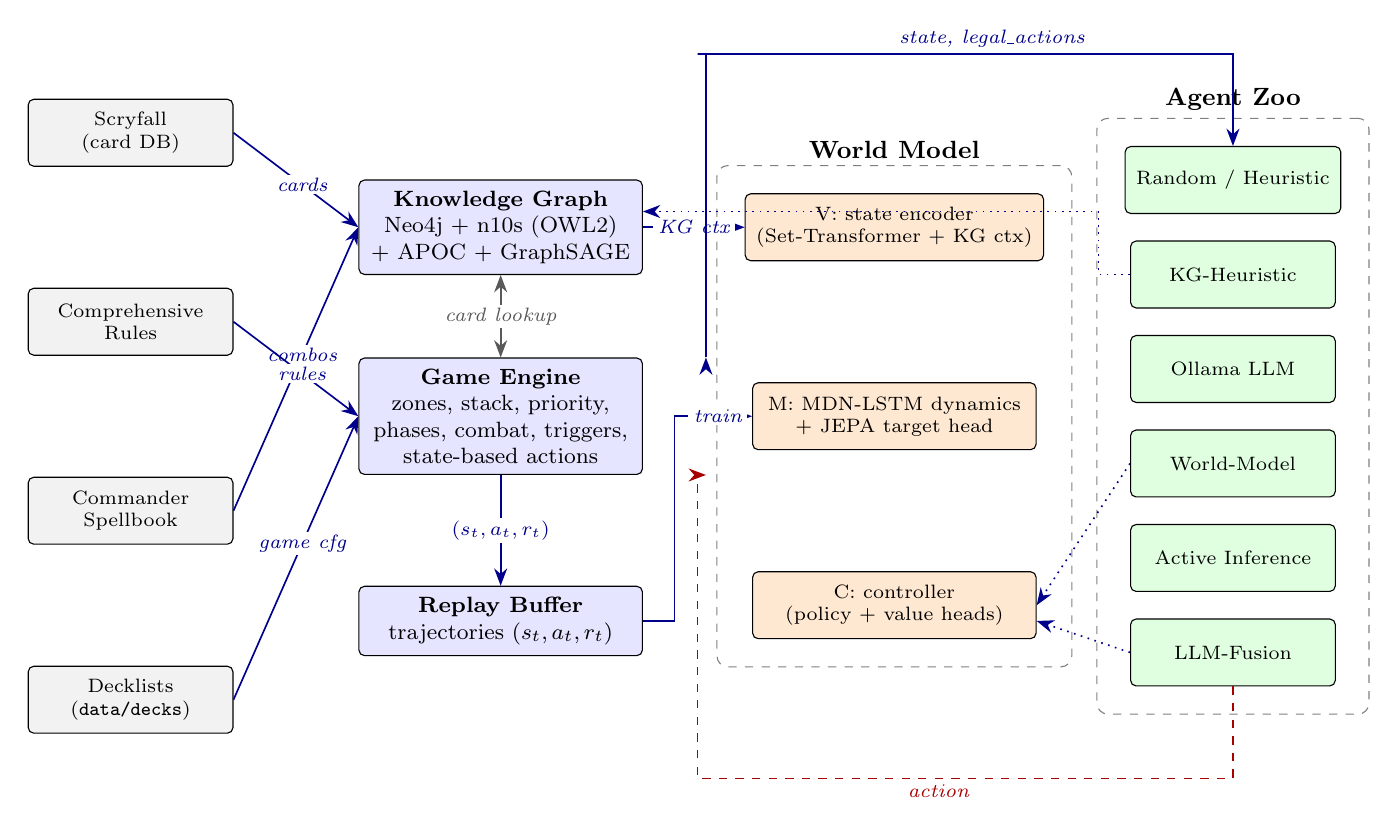
\begin{tikzpicture}[
    >={Stealth[length=2.2mm]},
    font=\footnotesize,
    box/.style ={draw, rounded corners=2pt, align=center,
                 minimum height=0.85cm, inner sep=4pt},
    data/.style={box, fill=gray!10,    minimum width=2.6cm, font=\scriptsize},
    sym/.style ={box, fill=blue!10,    minimum width=3.6cm},
    learn/.style={box, fill=orange!18, minimum width=3.6cm, font=\scriptsize},
    agent/.style={box, fill=green!12,  minimum width=2.6cm, font=\scriptsize},
    grp/.style ={draw=black!50, dashed, rounded corners=4pt, inner sep=10pt},
    flow/.style={->, semithick, blue!55!black},
    twoway/.style={<->, semithick, gray!70!black},
    backflow/.style={->, semithick, dashed, red!65!black},
    elabel/.style={font=\scriptsize\itshape, fill=white,
                   inner xsep=2pt, inner ysep=1pt}
  ]

  % ---- Column 1: data sources (well-spaced, no overlap) -----------------
  \node[data] (scry)  at (0,  3.6) {Scryfall\\(card DB)};
  \node[data] (rules) at (0,  1.2) {Comprehensive\\Rules};
  \node[data] (sb)    at (0, -1.2) {Commander\\Spellbook};
  \node[data] (decks) at (0, -3.6) {Decklists\\(\texttt{data/decks})};

  % ---- Column 2: symbolic substrate ------------------------------------
  \node[sym] (kg)  at (4.7,  2.4) {\textbf{Knowledge Graph}\\
        Neo4j + n10s (OWL2)\\+ APOC + GraphSAGE};
  \node[sym] (eng) at (4.7,  0.0) {\textbf{Game Engine}\\
        zones, stack, priority,\\phases, combat, triggers,\\state-based actions};
  \node[sym] (rb)  at (4.7, -2.6) {\textbf{Replay Buffer}\\trajectories $(s_t,a_t,r_t)$};

  % ---- Column 3: world model V/M/C ------------------------------------
  \node[learn] (V) at (9.7,  2.4) {V: state encoder\\(Set-Transformer + KG ctx)};
  \node[learn] (M) at (9.7,  0.0) {M: MDN-LSTM dynamics\\+ JEPA target head};
  \node[learn] (C) at (9.7, -2.4) {C: controller\\(policy + value heads)};
  \begin{pgfonlayer}{background}
    \node[grp, fit=(V)(M)(C),
          label={[font=\small\bfseries, yshift=-1pt]above:World Model}] (wm) {};
  \end{pgfonlayer}

  % ---- Column 4: agents ------------------------------------------------
  \node[agent] (a1) at (14.0,  3.0) {Random / Heuristic};
  \node[agent] (a2) at (14.0,  1.8) {KG-Heuristic};
  \node[agent] (a3) at (14.0,  0.6) {Ollama LLM};
  \node[agent] (a4) at (14.0, -0.6) {World-Model};
  \node[agent] (a5) at (14.0, -1.8) {Active Inference};
  \node[agent] (a6) at (14.0, -3.0) {LLM-Fusion};
  \begin{pgfonlayer}{background}
    \node[grp, fit=(a1)(a6),
          label={[font=\small\bfseries, yshift=-1pt]above:Agent Zoo}] (agents) {};
  \end{pgfonlayer}

  % ---- data -> symbolic ------------------------------------------------
  \draw[flow] (scry.east)  -- node[elabel,pos=0.55]{cards}   (kg.west);
  \draw[flow] (sb.east)    -- node[elabel,pos=0.55]{combos}  (kg.west);
  \draw[flow] (rules.east) -- node[elabel,pos=0.55]{rules}   (eng.west);
  \draw[flow] (decks.east) -- node[elabel,pos=0.55]{game cfg}(eng.west);

  % ---- engine <-> KG (lookup) -----------------------------------------
  \draw[twoway] (kg.south) -- node[elabel]{card lookup} (eng.north);

  % ---- engine -> replay buffer ----------------------------------------
  \draw[flow] (eng.south) -- node[elabel]{$(s_t,a_t,r_t)$} (rb.north);

  % ---- training: replay -> M; KG -> V ---------------------------------
  \draw[flow] (rb.east) -- ++(0.4,0) |- node[elabel,pos=0.78]{train} (M.west);
  \draw[flow] (kg.east) -- node[elabel]{KG ctx} (V.west);

  % ---- agent decide_action loop -- routed in the COLUMN GAP between the
  % symbolic substrate (x=4.7) and the WM (x=9.7), then along far top/bottom
  % buses, so they never cross any node.
  \coordinate (busTop)  at (7.2,  4.6);
  \coordinate (busBot)  at (7.2, -4.6);
  \coordinate (busTopR) at (14.0, 4.6);
  \coordinate (busBotR) at (14.0,-4.6);

  \draw[flow]
      ([xshift=8mm]eng.north east) -- ++(0,0)
      coordinate (engUp);
  \draw[flow]
      (engUp) |- (busTop)
      -- (busTopR)
      node[elabel, pos=0.55, above=1pt]{state, legal\_actions}
      -- (a1.north);

  \draw[backflow]
      (a6.south) -- (busBotR)
      -- (busBot)
      node[elabel, pos=0.55, below=1pt]{action}
      |- ([xshift=8mm]eng.south east);

  % ---- agent lookups (dotted) -----------------------------------------
  \draw[flow, dotted] (a4.west) -- (C.east);
  \draw[flow, dotted] (a6.west) -- ([yshift=-2mm]C.east);
  \draw[flow, dotted] (a2.west) -- ++(-0.4,0) |- ([yshift=2mm]kg.east);

\end{tikzpicture}
\end{document}
